% This is samplepaper.tex, a sample chapter demonstrating the
% LLNCS macro package for Springer Computer Science proceedings;
% Version 2.21 of 2022/01/12
%
\documentclass[runningheads]{llncs}
%
\usepackage[T1]{fontenc}
% T1 fonts will be used to generate the final print and online PDFs,
% so please use T1 fonts in your manuscript whenever possible.
% Other font encondings may result in incorrect characters.
%
\usepackage{graphicx}
% Used for displaying a sample figure. If possible, figure files should
% be included in EPS format.
%
% If you use the hyperref package, please uncomment the following two lines
% to display URLs in blue roman font according to Springer's eBook style:
%\usepackage{color}
%\renewcommand\UrlFont{\color{blue}\rmfamily}
%\urlstyle{rm}
%
\begin{document}
%
\title{Reducing Intuitive-Physics Prediction Error through Playing}
%
\titlerunning{Reducing Prediction Error through Playing}
% If the paper title is too long for the running head, you can set
% an abbreviated paper title here
%
\author{Olivier L. Georgeon\inst{1, 2}\orcidID{0000-0003-4883-8702} \and
Paul Robertson\inst{3}\orcidID{0000-0002-4477-0379} }
%
\authorrunning{Georgeon and Robertson}
% First names are abbreviated in the running head.
% If there are more than two authors, 'et al.' is used.
%
\institute{UR CONFLUENCE: Sciences et Humanites (EA 1598), UCLy, France 
	\email{ogeorgeon@univ-catholyon.fr} \and
SyCoSMA, LIRIS, CNRS, Villeurbanne, France \and
DOLL Labs, Lexington, MA, USA\\
\email{paulr@dollabs.com}}
%
\maketitle              % typeset the header of the contribution
%
\begin{abstract}
We present a method for an autonomous robot to generate behaviors to calibrate its intuitive-physics engine also known as the ``Game Engine in the Head'' (GEITH).
%The robot selects behaviors that yield information to refine the GEITH parameters. 
At the beginning of each interaction cycle, the robot uses its GEITH to run a simulation to compute predicted sensory signals. 
For each sensor, prediction error is the difference of the predicted sensory signal minus the actual sensory signal received at the end of the interaction cycle. 
Results show that over a few tens of interaction cycles, the robot improves its GEITH calibration and decreases its prediction errors. 
Moreover, the robot generates behaviors that human observers describe as playful.

\keywords{Active infernce  \and constructivist learning \and enaction \and intrinsic motivation \and robotics \and core knowledge.}
\end{abstract}
%
%
%
\section{Introduction}

It is widely believed that cognitive beings possess some kind of a \textit{world model} that they use to generate intelligent behaviors.
How they construct, maintain, and use this world model remains, however,  an open question in cognitive science and artificial intelligence. 

Karl Friston and his research group have proposed Active Inference \cite[e.g.]{smith_step-by-step_2022} as a method to infer the world model by minimizing \textit{free energy} \cite{friston_free-energy_2010}.
The world model at step $t$ is represented as a probability distribution $\mu_t$ that give the probability of being in any world state $s \in S$. 
This method iteratively updates $\mu_t$ on each interaction cycle.
The agent selects the action that is expected to maximize the information gained. 
The estimation of expected information gained is computed through the variational free energy which involves a divergence between two probability distributions: the agent's world model $\mu$ and the joint probability distribution $g = P(O, S)$ of observations $O$ and world states $S$ called the \textit{generative model}. 
This method, however, requires that the set of states $S$ and the relations between states and observations $O$ be known \textit{a prior}. 
Moreover, the high computational requirements to compute the free energy and the high number of interaction cycles to converge to a useful world model makes this method inapplicable in our case of a robot interacting with the open world. 

The Partially Observable Markov Decision Process (POMDP) literature proposes a broad range of methods to infer a \textit{belief state} in a partially observable process.
The belief state amounts to the agent's world model of the environment that the agent can only partially observe.  
If the state transition function and the observation function are known \textit{a priori}, the problem of computing the belief state has been mathematically solved \cite{astrom1965optimal}. 
It was also proven that the implementation of the solution becomes intractable as the set of states and observation grows. 
Without knowledge of the state transition and observation functions, the problem of inferring belief states in POMDPs does not lend itself to a mathematical analysis. 

The active inference and the POMDP literature suggests that inferring the world model through experience of interaction requires prior assumptions to reduce complexity. 
The present study proposes the hypothesis that the ``Game Engine In The head'' (GEITH) can work as a suitable prior assumption. 

Joshua Tenenbaum and his research group have proposed the GEITH \cite{battaglia_simulation_2013} as the capacity of cognitive beings to simulate basic dynamics of physics and interactions. 
In mammals, the GEITH would rest upon brain structures that are partially predefined by genes and then completed through ontogenetic development.  
Similarly, it is possible to endow artificial agents and robots with a predefined software game engine, and expect them to refine the parameters of their game engine as they test their predictions in the world.

The refinement of the game engine is measured through two methods. 
The first is performed by the robot itself by measuring the prediction error of sensory signals. 
Decrease in prediction errors shows improvement of the game engine. 
The second is performed by the experimenter by assessing whether the game engine parameters converge towards a target range that indicates that the robot managed to calibrate its GEITH. 




\section{Our hypothesis}

For an extended argumentation on our theoretical positioning we refer the reader to our previous article \cite{georgeon_artificial_2024}.
We investigate the core knowledge system \cite{spelke_core_2012}.
We implement an emotional system \cite{chebotareva_emotional_2019} based on three main neurotransmitters: dopamine, serotonin, and noradrenaline.
The robot must follow a chain of causality to explain the prediction errors \cite{thorisson_explanation_2021}.

\begin{figure}
	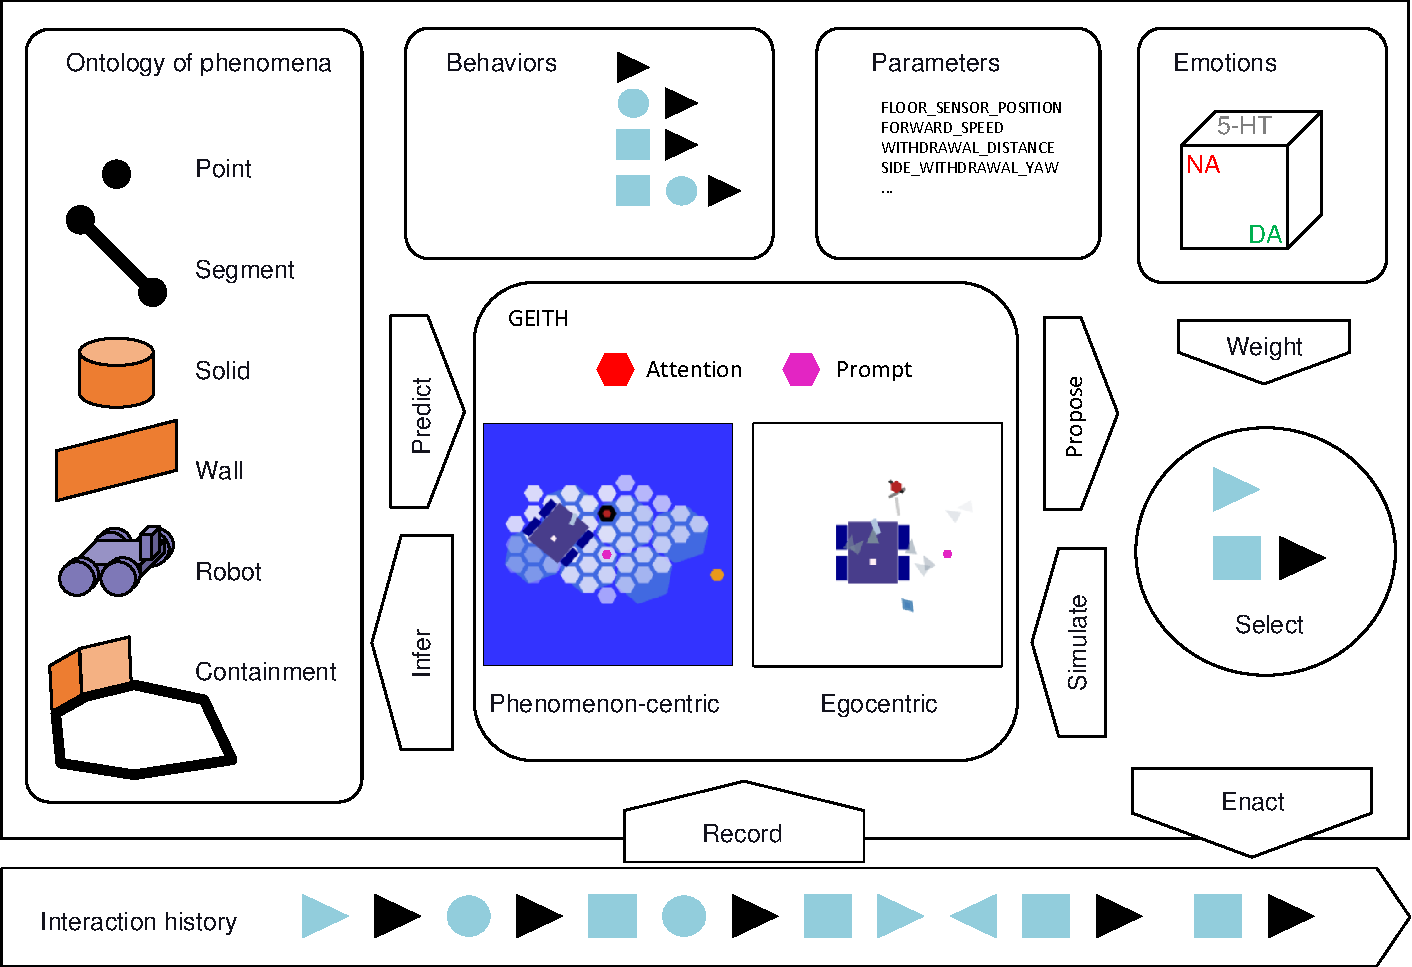
\includegraphics[width=\textwidth]{Figure_geith.pdf}
	\caption{The game engine within the robot's cognitive architecture.
	Bottom: the history of interactions enacted over time.
	Center: the working memory that implements the game engine and proposes future behaviors.
	Left: the types of phenomena inferred trough interactive experience.
	Top center: set of behaviors.
	Top right: The three-dimensional emotional state based on Dopamine (DA), Serotonin (5-HT), and Noradrenaline (NA) levels.
	Right: the decider selects the next behavior based on the emotional state and the expected outcome predicted from simulation.} \label{fig:geith}
\end{figure}



\section{Experiment}

The robot is based on the Osoyoo robot car \cite{osoyoo_robot_car}.
The code is open source and shared online \cite{petitcat_github}.

\begin{figure}
	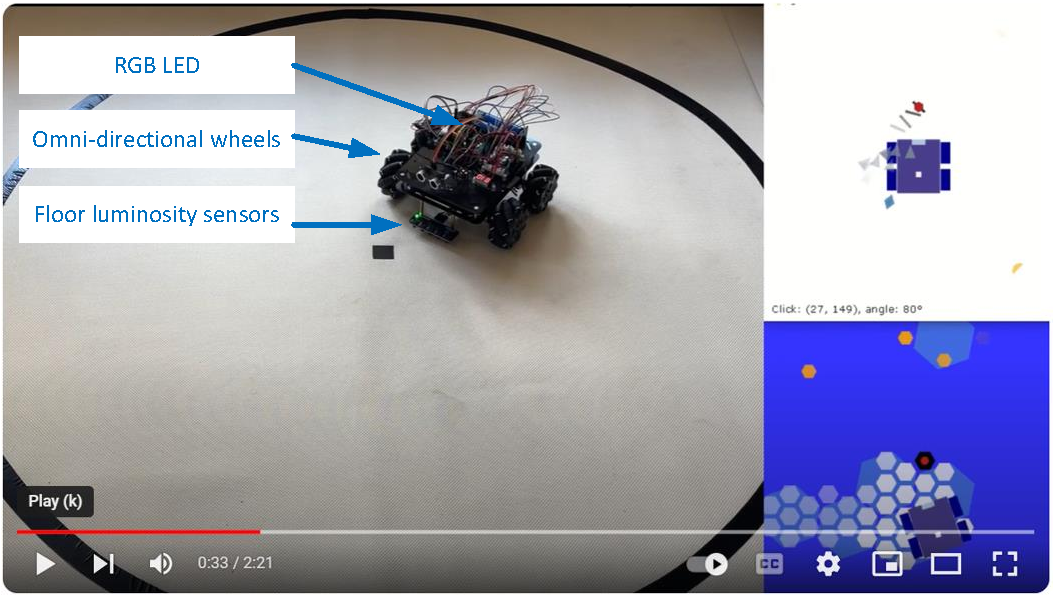
\includegraphics[width=\textwidth]{Figure_video.pdf}
	\caption{Screenshot of a video example run \cite{georgeon_petitcat_2024}.
	Left: the robot playing with a dot on the floor.
	Top right: the robot's egocentric memory. Black segments: events of interaction with the black dot. 
	Bottom right: allocentric memory. Black hexagon: the black dot used as a point of reference. Yellow hexagons: echo measured with the sonar. Red hexagon: the robot's focus of attention.} \label{fig:video}
\end{figure}


% \subsection{The robotics platform}

% \subsection{The Game Engine In The Head}

\section{Results}

Several videos are available online. Here we analyze \cite{georgeon_petitcat_2024}.

\begin{figure}
	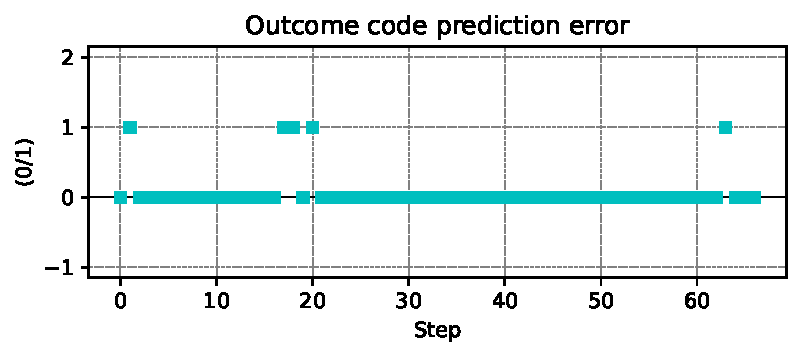
\includegraphics[width=\textwidth]{01_Outcome_code.pdf}
	\caption{Prediction error of black line detection.
	Step 2: the robot did not expect to detect the dot.
	Steps 17: the robot expected to detect the dot while translating forward but missed it.
	Steps 18: the robot expected to not detect the dot while turning around but detected it.
	Step 20: the robot did not predict detecting the dot through simulation but it did. 
	Step 65: The robot did not expect to detect the surrounding arena. } \label{fig:yaw_pe}
\end{figure}

\begin{figure}
	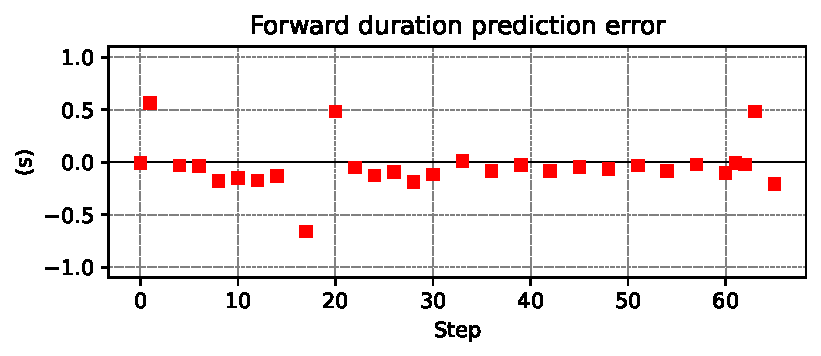
\includegraphics[width=\textwidth]{07_Forward_duration_pe.pdf}
	\caption{Move forward duration prediction error.
	Step 2 and 20: the forward translation was unexpectedly interrupted by the dot detection.
	Step 17: the forward duration was longer than expected because the robot did not detect the dot.
	From Step 21 to 64: forward duration prediction error slightly decreases. 
	Step 65: the forward translation was unexpectedly interrupted by the detection of the arena border.} \label{fig:yaw_re}
\end{figure}


\begin{figure}
	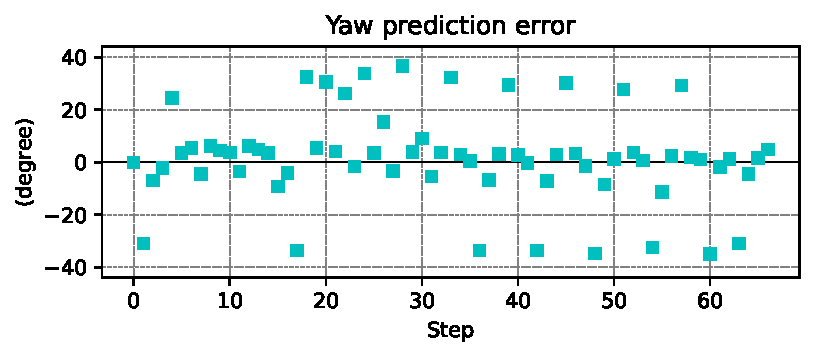
\includegraphics[width=\textwidth]{02_yaw_pe.pdf}
	\caption{The yaw prediction error shows no significant trend when we do not distinguish between the different kinds of interactions.} \label{fig:yaw_pe}
\end{figure}

\begin{figure}
	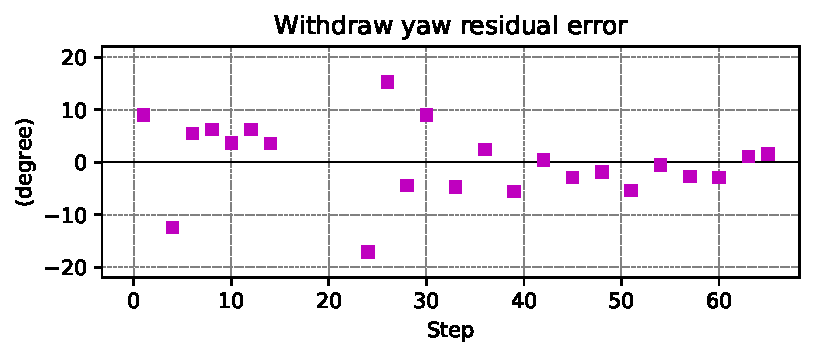
\includegraphics[width=\textwidth]{03_yaw_re.pdf}
	\caption{The yaw residual error during interactions in which the robot detects the dot decreases significantly after Step 26.} \label{fig:yaw_re}
\end{figure}

\begin{figure}
	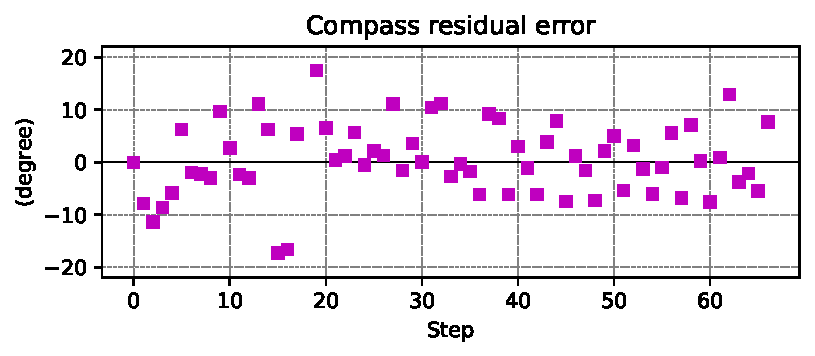
\includegraphics[width=\textwidth]{04_Compass.pdf}
	\caption{The compass residual error decreases after step 20 when the robot starts circling around the dot.
	It nonetheless remains noisy due to sensor imprecision.
	The sliding average over 10 interactions tends to 0.8° and the standard deviation to 7.4°.} \label{fig:compass}
\end{figure}

\section{Conclusion}


\begin{credits}

%\subsubsection{\ackname} A bold run-in heading in small font size at the end of the paper is
%used for general acknowledgments, for example: This study was funded
%by X (grant number Y).

%\subsubsection{\discintname}
%It is now necessary to declare any competing interests or to specifically
%state that the authors have no competing interests. Please place the
%statement with a bold run-in heading in small font size beneath the
%(optional) acknowledgments\footnote{If EquinOCS, our proceedings submission
%system, is used, then the disclaimer can be provided directly in the system.},
%for example: The authors have no competing interests to declare that are
%relevant to the content of this article. Or: Author A has received research
%grants from Company W. Author B has received a speaker honorarium from
%Company X and owns stock in Company Y. Author C is a member of committee Z.
\end{credits}
%
% ---- Bibliography ----
%
% BibTeX users should specify bibliography style 'splncs04'.
% References will then be sorted and formatted in the correct style.
%
\bibliographystyle{splncs04}
\bibliography{georgeon.bib}
%
\end{document}
